\documentclass{article}
\usepackage{graphicx}
\usepackage{caption}
\usepackage{subcaption}

\author{Ruben Sharpe}
\title{Crime and the city:\\Spatial planning for crime reduction}
\date{\today}

\begin{document}
\maketitle

\begin{abstract}
 It is hypothesised that crime in a neighbourhood is correlated, albeit in a complex manner with the availability of public venues. Rather than hypothesising about causal relations, a machine learning approach is proposed in which high-crime, medium-crime and low-crime neighbourhoods are characterised by their public venues. These characterisations may serve as templates for good and bad practices in spatial planning.
 As a test case, the city of Tornonto (Ontario, Canada) was characterised based on information about public venues, obtained from Foursquare, and the City government of Toronto Open Dataset on crime. 
 
 Neighbourhoods were clustered by similarity of their composition in terms of venues using K-means clustering.  
 Spatial information on crime was visualised in choropleth maps of Toronto. Visual comparison of neighbourhood clusters with crime maps shows the feasibility of the approach.
 
 Decision trees and support vector machines were trained to classify neighbourhoods as high-, medium- or low-crime. With such models, city planners may try to predict how modifications would impact the crime classification or,in other words, which modifications correlate with what crime level.
\end{abstract}

\tableofcontents



\section{Introduction}
It is intuitively clear that public venues, such as bars and restaurants, but also public service locations such as transport hubs or banks impact the wellbeing of local communities. However, it is not straightforward to predict whether this impact will be positive or negative.Bars and restaurants can enliven a neighbourhood and may contribute to greater safety because of increased presence of people in the streets, because potential witnesses deter crime. On the other hand, the presence of bars and restaurants is also correlated with alcohol abuse related crime. Similarly, there is a duality in the social impact for the presence of shops and banks. These may have a positive impact because of associated prosperity, but may also attract criminal activity at night because of reduced traffic compared to residential areas.\\

The complexity and the interrelatedness of these issues carries over to the complexity of city planning. The difficulty for city planners, moreover, is that they rarely get to design a neighbourhood from scratch. Typically, they have to deal with neighbourhoods with for the most part a fixed set of public facilities, and which may be suboptimal from a design point of view. The question for a city planner, therefore, is often : ``What would be, \emph{for a certain neighbourhood and given all its other attributes}, the impact of building (or removing) a shopping mall? Or a park? Or adding, or removing a bus stop?''\\

There is, of course, a lot of scientific literature on this topic but that is out of the scope of this project. This report is aimed at city planners and is intended to show the feasibility of machine learning as a tool for spatial planning.\\
Machine learning allowes an automated approach to compare neighbourhoods both in terms of their public venues and in terms of social markers, such as crime rates. This provides city planners, apart from their professional expertise, with examples of good and bad practices that may help them in their decision making.\\
For reasons of convenience, the analysis in this report will look at the city of Toronto (Ontario, Canada). Crime rates will be used as the proxy for the wellbeing of communities, although other markers such as employment rate or health statistics could also be used.

\section{Data}
Location data, information about public venues and crime statistics will be used to classify neighbourhoods and map them with respect to the prevalance of crime. From this, generalised conclusions may be drawn with respect to the makeup of `high-crime' and `low-crime' neighbourhoods. 

% An example of a map of the geographical location of similar neighbourhoods, which can be mapped onto crime information, is given in Figure \ref{fig:clustermap}. An example of the characterisation of one of such clusters is given in Figure \ref{fig:cluster}
% \begin{figure}[h]
%  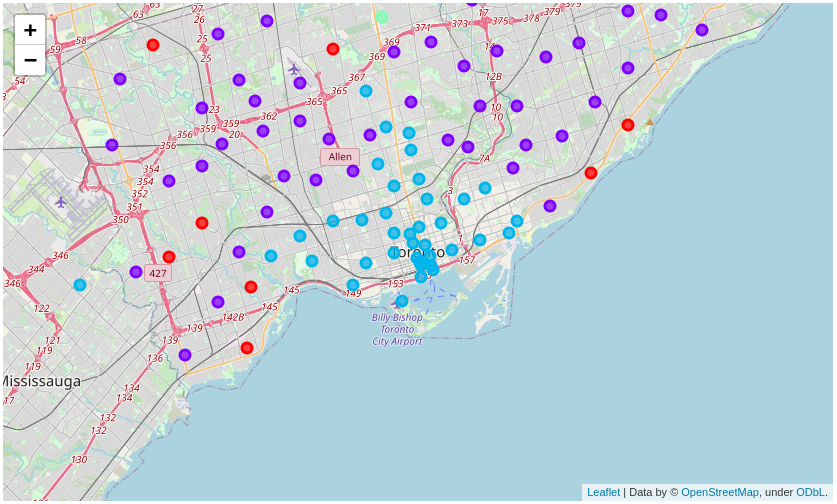
\includegraphics[width=\textwidth]{pics/clustermap.png}
%  \caption{Example the clustering of similar neighbourhoods in Toronto. Similar colours denote similar neighbourhoods.}\label{fig:clustermap}
% \end{figure}
% \begin{figure}[h]
%  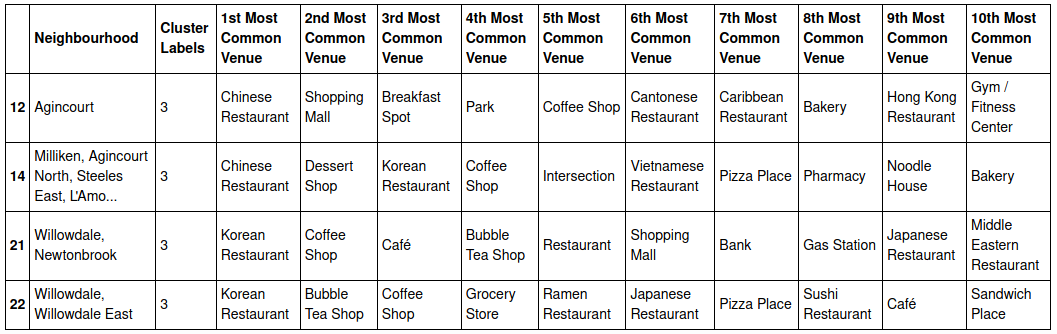
\includegraphics[width=\textwidth]{pics/cluster.png}
%  \caption{Example of a cluster of similar neighbourhoods. Note that the most prevalent venues are Asian restaurants.}\label{fig:cluster}
% \end{figure}


\subsection{Location data}
Location data for the city of Toronto can be acquired by scraping postal codes, boroughs and neighbourhoods from Wikipedia.\footnote{https://en.wikipedia.org/wiki/List\_of\_postal\_codes\_of\_Canada:\_M} This data needs to be  enriched with the GPS coordinates of the respective neighbourhoods. These coordinates can be obtained from the internet in the form of a `.csv' file from the Coursera website for the Data Science Capstone.\footnote{https://cocl.us/Geospatial\_data} The enriched dataset consists of the postal codes, borough, and neighbourhood names and the neighbourhoods' latitude and longitude (Figure \ref{fig:enriched}).
% \begin{table}[ht]
% \centering
%     \begin{tabular}{l}
%     \hline\hline
%         Postal Code\\
%         Borough\\
%         Neighbourhood\\
%         Latitude\\
%         Longitude\\
%     \hline
%     \end{tabular}\caption{Toronto location data (103 postal codes for 140 neighbourhoods in 11 boroughs).}\label{tab:locations}
% \end{table}

% \begin{figure}[h]
%  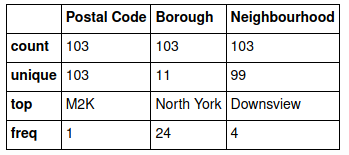
\includegraphics[width=6cm]{pics/scraped.png}
%  \caption{Example of cleaned data after scraping from Wikipedia.}
%  \label{fig:locations}
% \end{figure}
\begin{figure}[ht]
 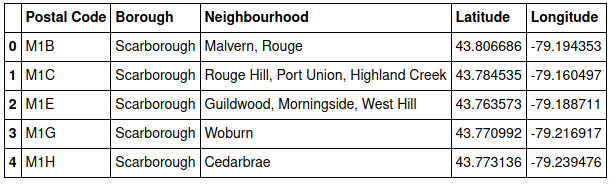
\includegraphics[width=\textwidth]{pics/enriched.png}
 \caption{Example of data enriched with coordinates.}
 \label{fig:enriched}
\end{figure}


\subsection{Public venues}
Foursquare is used to obtain information about the public venues, specifically their category, in each neighbourhood (Figure \ref{fig:venues}). For this purpose, the neighbourhood is arbitrarily defined as the area within a 1.500 m radius around a postal code's geographical centre. The top 10 most prevalent venues will be used to characterise the neighbourhood (Figure \ref{fig:grouped}).
% \begin{table}[ht]
% \centering
%     \begin{tabular}{l}
%     \hline\hline
%         Neighbourhood\\
%         Neighbourhood Latitude\\
%         Neighbourhood Longitude\\
%         Venue\\
%         Venue Latitude\\
%         Venue Longitude\\
%         Venue Category\\
%     \hline
%     \end{tabular}
% \caption{Venue data (6884 venues, 349 unique venue categories for 140 neighbourhoods in 99 postal code areas).}\label{tab:venues}
% \end{table}
\begin{figure}[ht]
 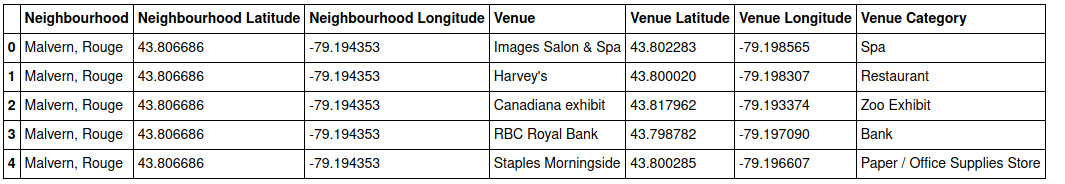
\includegraphics[width=\textwidth]{pics/venues.png}
 \caption{Example of which venue information can be obtained.}\label{fig:venues}
\end{figure}
\begin{figure}[ht]
 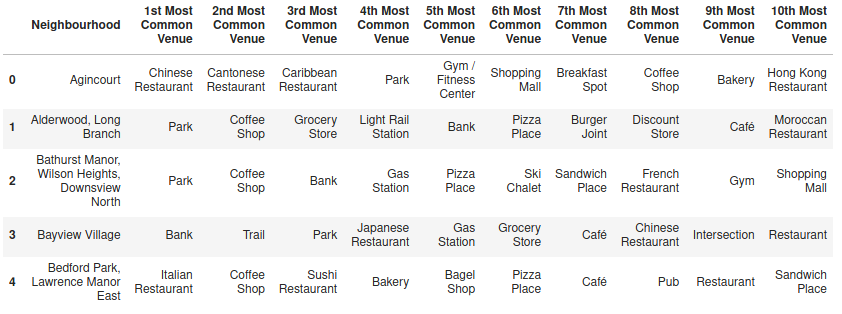
\includegraphics[width=\textwidth]{pics/grouped.png}
 \caption{Example of neighbourhoods with top 10 most prevalent venues.}\label{fig:grouped}
\end{figure}

\subsection{Crime data}
The city of Toronto provides a lot of open data related to the city.\footnote{https://www.toronto.ca/city-government/data-research-maps/open-data/} This data ranges from polls conducted by the government, to inventory lists of street furniture, to `bicycle count and locations' and is ever increasing. From this repository, a list of crime rates can be obtained.\footnote{https://open.toronto.ca/dataset/neighbourhood-crime-rates/} This list contains, for each neighbourhood the number of incidences of certain types of crime (Table \ref{tab:crime}). Population information from the 2016 census, included in the file, can be used to normalise crime rates relative to population size. Conveniently, the file also contains geographical information so that this information can be easily mapped. The crime categories that are accessible from the data files are given in Table \ref{tab:crime}.
\begin{table}[ht]
\centering
    \begin{tabular}{ll}
    \hline\hline
        Assault &  from 2014 -- 2019\\
        Auto Theft &  from 2014 -- 2019\\
        Breaking and Entering &  from 2014 -- 2019\\
        Homicide &  from 2014 -- 2019\\
        Robbery &  from 2014 -- 2019\\
        Theft &  from 2014 -- 2019\\
    \hline
    \end{tabular}
\caption{Crime data categories.}\label{tab:crime}
\end{table}
% \begin{figure}
%  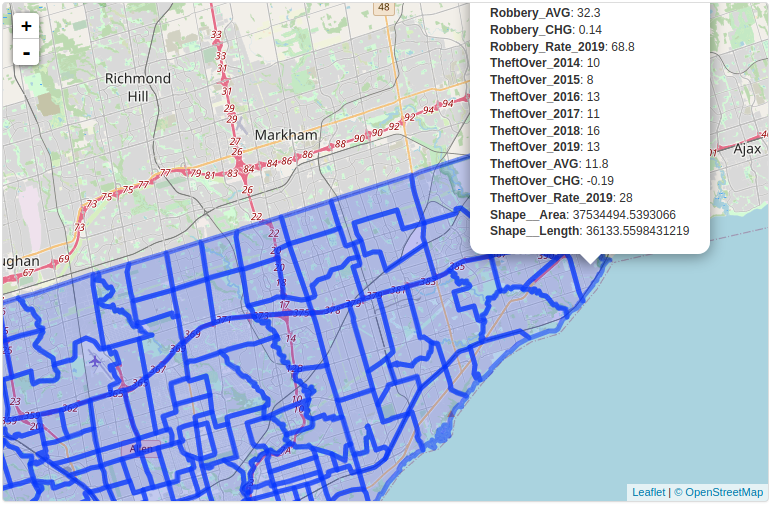
\includegraphics[width=\textwidth]{pics/crime.png}
%  \caption{Example of crime information can be obtained in conjunction with a geographical location. Image is generated from the Toronto city government website.}\label{fig:crime}
% \end{figure}


\section{Methodology}
\subsection{Exploration of crime information}
Crime information is available for six categories. This information may be visualised in choropleth maps (Figure \ref{fig:assault}). For direct comparison with the neighbourhood information, the neighbourhood names in both datasets must be correlated.
\begin{figure}[ht]
 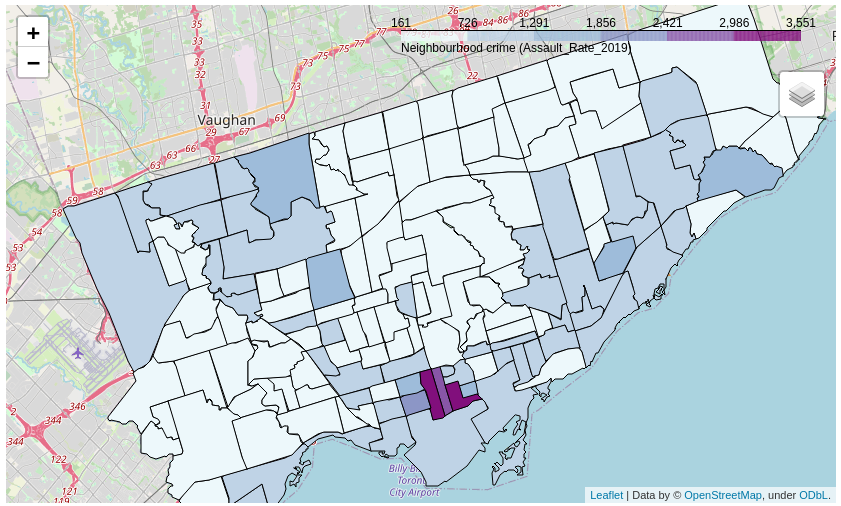
\includegraphics[width=\textwidth]{pics/assault.png}
 \caption{Choropleth map of assaults in 2019.}\label{fig:assault}
\end{figure}
% The neighbourhood names in the dataset with the geographical information (which includes the venue information) have been organised by postal code. Since some neighbourhoods share the same postal code these need to be expanded for comparison with the crime data (Figure \ref{fig:expanded}).
% \begin{figure}[ht]
%      \centering
%      \begin{subfigure}[b]{0.55\textwidth}
%          \centering
%          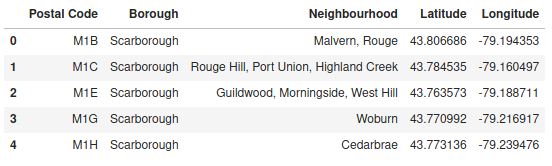
\includegraphics[width=\textwidth]{pics/names}
%          \caption{Before}
%      \end{subfigure}
%      \hfill
%      \begin{subfigure}[b]{0.4\textwidth}
%          \centering
%          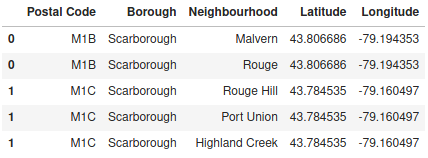
\includegraphics[width=\textwidth]{pics/exploded}
%          \caption{After}
%      \end{subfigure}
%         \caption{Difference in dataset before, and after expanding.}
%         \label{fig:expanded}
% \end{figure}
However, upon joining the dataset for the geographical data with that for the crime data, it is found that the names are so dissimilar that only 20 neighbourhoods are found to match up (Figure \ref{fig:dissimilar}).\footnote{This is true, even after the individual neighbourhood names were reconstituted from those that were originally combined because they share the same postal code.} Fortunately, the Toronto city government provides a `geojson' file for the crime data so that neighbourhood information and crime information may be mapped, independently of each other. This allows their visual inspection and subsequent manual labeling of neighbourhoods in the venue dataset with respect to `crime proneness' (Figure \ref{fig:manual}). 
\begin{figure}[ht]
\centering
 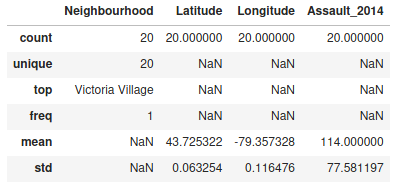
\includegraphics[width=0.6\textwidth]{pics/dissimilar.png}
 \caption{Statistical information of the dataset after an `inner' merge of geographical and crime datasets. Note the count of only 20 neigbourhoods in stead of the expected 140.}\label{fig:dissimilar}
\end{figure}
\begin{figure}[ht]
 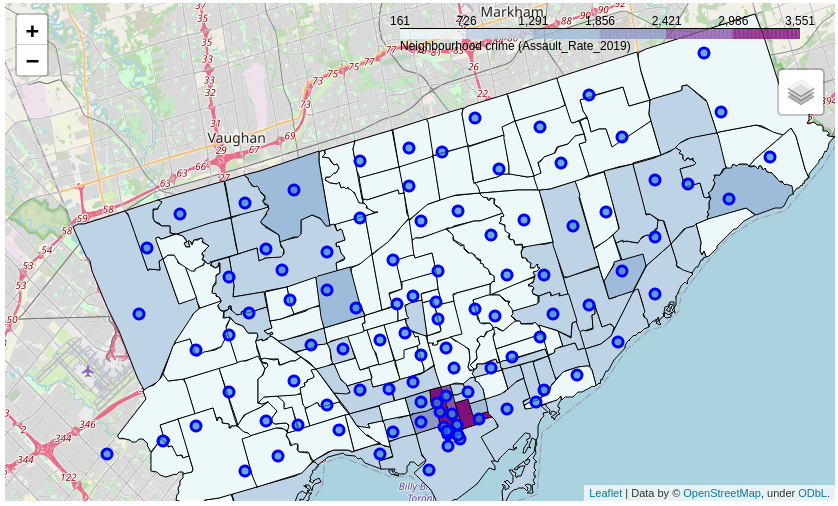
\includegraphics[width=\textwidth]{pics/manual.png}
 \caption{Crime (assault) choropleth, plotted together with neighbourhood information. Neighbourhoods (dots) that lie on purple areas may be manually labeled 'high-crime', neighbourhoods on blue areas `medium-crime' and neighbourhoods on light blue areas `low-crime'.}\label{fig:manual}
\end{figure}

Since there are six crime categories, a neighbourhood classification in `high-', `medium-' or `low-crime' must either relate to one of the six categories or a new crime index must be constructed. For this, each crime category is first normalised with respect to the maximum number of occurences across all neighbourhoods. Then these indices are summed over all the six crime categories and normalised again with respect to the maximum of this new `overall' category. This can be interpreted as follows: an index of `1' means that the neigbourhood has scored, on average, the worst in all crime categories, whereas an index of `0' means that there have been no incidences of crime in any of the categories in that neighbourhood. When using the crime \emph{rate} for each crime category, these are already represented as incidents per 100.000 population and therefore the population size of each neigbourhood does not need to be taken into account.

\subsection{Machine learning}
\subsubsection{Exploration of neighbourhood clusters}
Data exploration is done mostly by visual inspection. Similarity of neighbourhoods with respect to their public venues, as well as the spatial distribution of similar neighbourhoods is explored using K-means clustering. The number of clusters is arbitrary so it is good to get an idea of the inner-cluster cohesion by inspecting the output of the clustering algorithm for increasing numbers of clusters. From this, it can be observed which clusters break up first and which stay in tact, thereby indicating a greater dissimilariy with respect to the other clusters. Comparison of clusters with the spatial distribution of crimes may give an indication of how these are correlated.

\subsubsection{Modelling}
K-means clustering provides some qualitative insight in the correlation between neighbourhood composition and the occurence of crime. Clusters of neighbourhoods may therefore be classified according to some crime rating (e.g. high-, medium- and low-crime). This classification, however, is not inherent in K-means clustering. It only takes into account similarity and dissimilarty of neigbourhoods, not how well this correlates with crime. It is, moreover, not necessarily obvious how changes in the neighbourhood composition may cause this classification to change. In other words, it is from K-means clustering not obvious which changes would cause a certain neighbourhood to become more or less similar neighbourhoods with a more desirable crime rating. For this reason, a decision tree model will be built. Such a model will allow parsing of changes to a neighbourhood's composition and a prediction of the new crime rating. Decision trees are very intuitive and from its explicit structure it is easy extimate up front to which changes the outcome will be most sensitive to. For reasons of comparison, however, a support vector machine classifier will also be built.

\section{Results}
\subsection{Visual inspection}
Neighbourhoods in Toronto can, based on their public venues, broadly be grouped into two categories: one centred around the harbour and one broad band from east to west (Figure \ref{fig:nbhclusters}). From inspection of the most prevalent venues in each cluster, it is not intuitively clear how these clusters differ from one another (Figure \ref{fig:composition}).
\begin{figure}[ht]
     \centering
     \begin{subfigure}[b]{0.47\textwidth}
         \centering
         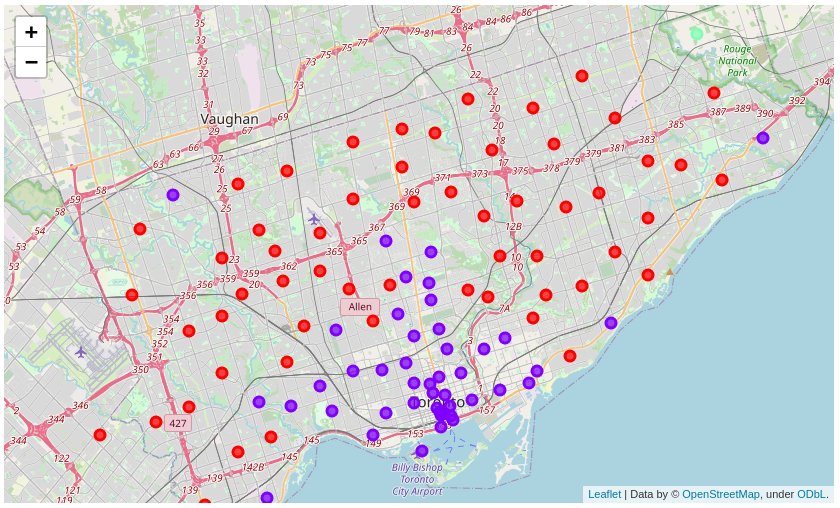
\includegraphics[width=\textwidth]{pics/clusters3}
         \caption{Three clusters}
     \end{subfigure}
     \hfill
     \begin{subfigure}[b]{0.47\textwidth}
         \centering
         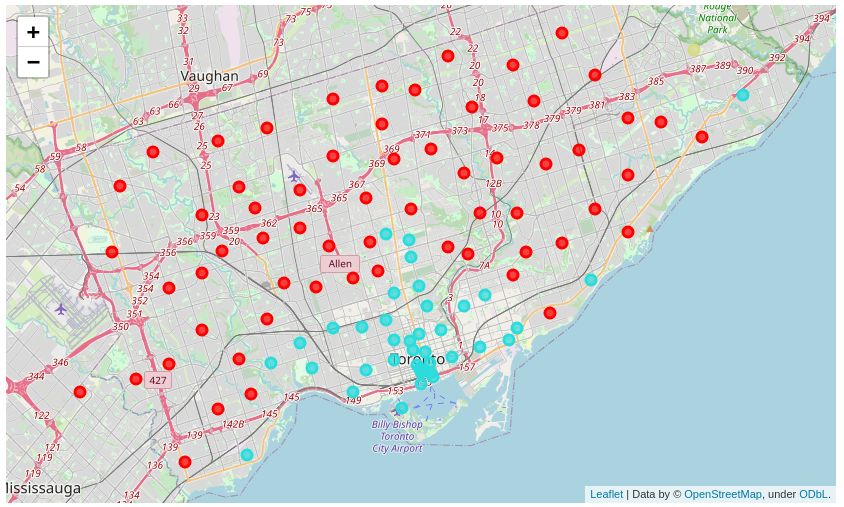
\includegraphics[width=\textwidth]{pics/clusters4}
         \caption{Four clusters}
     \end{subfigure}
     \begin{subfigure}[b]{0.47\textwidth}
         \centering
         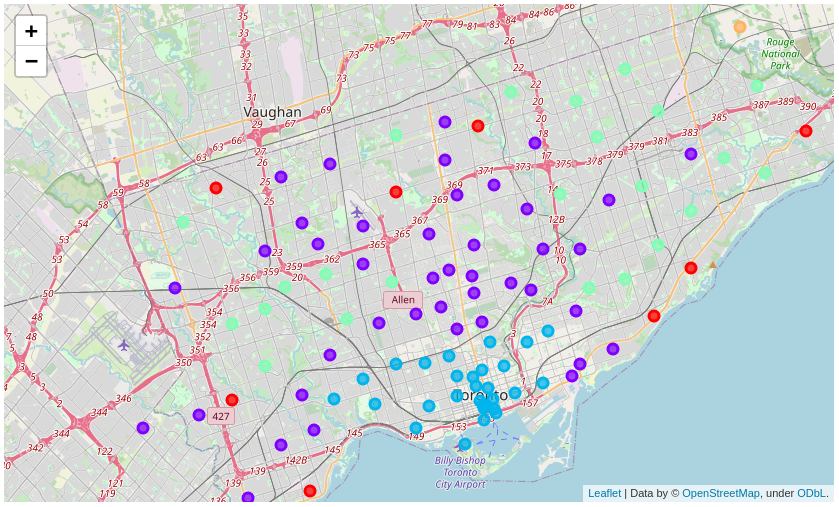
\includegraphics[width=\textwidth]{pics/clusters5}
         \caption{Five clusters}
     \end{subfigure}\hfill
     \begin{subfigure}[b]{0.47\textwidth}
         \centering
         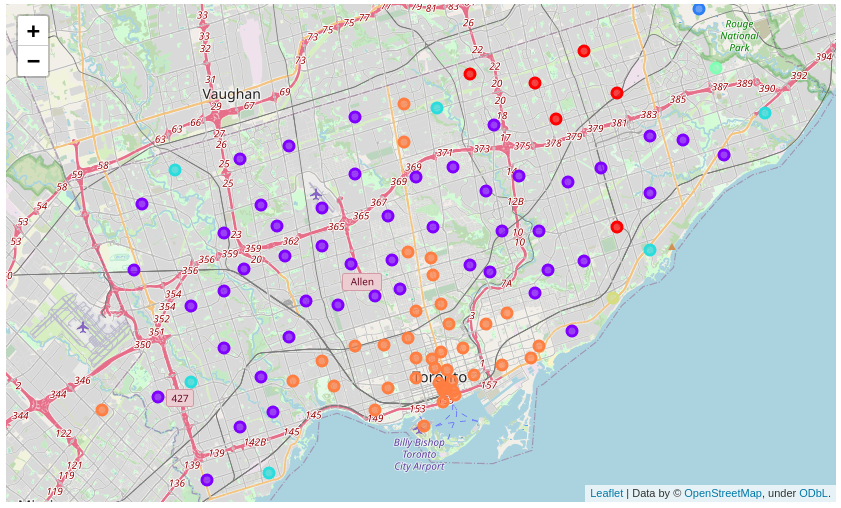
\includegraphics[width=\textwidth]{pics/clusters7}
         \caption{Seven clusters}
     \end{subfigure}
     \caption{Different distributions of three, four, five and seven clusters. Note that there are basically two stable clusters, concentrically oriented around the harbour. Increasing the number of clusters only causes small split offs.}
        \label{fig:nbhclusters}
\end{figure}

\begin{figure}[ht]
     \centering
        \begin{subfigure}[b]{\textwidth}
            \centering
            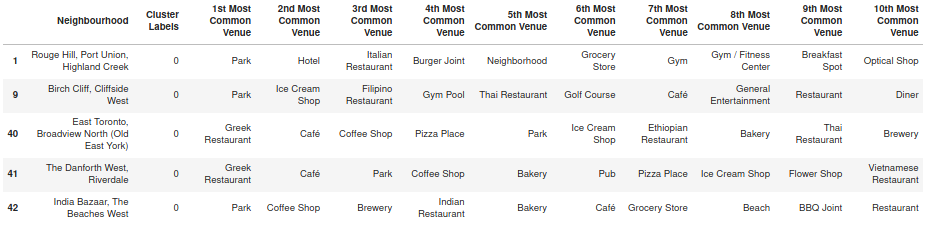
\includegraphics[width=\textwidth]{pics/composition_0}
            \caption{Venue composition of first five neighbourhoods in the `harbour' cluster.}
        \end{subfigure}
        \begin{subfigure}[b]{\textwidth}
            \centering
            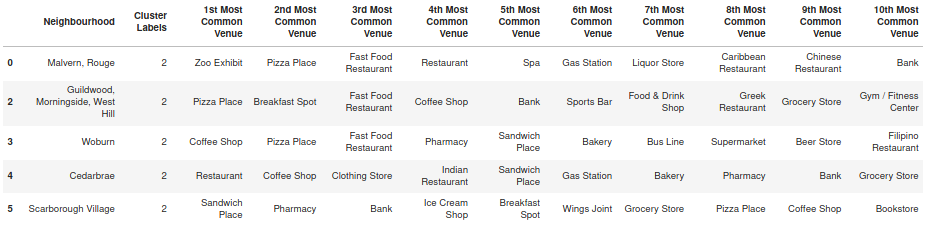
\includegraphics[width=\textwidth]{pics/composition_2}
            \caption{Venue compostition of the first five neighbourhoods in the `broad band' cluster.}
        \end{subfigure}
        \caption{Compositions of the most stable clusters. Note that although these are stable and therefore very dissimilar, the dissimilarity is not intuitively obvious.}
        \label{fig:composition}
\end{figure}

Spatially, the clusters correlate somewhat with the crime map, insofar that a relatively high crime index is found in the neighbourhoods around the harbour and in the North-West corner of Toronto. This agrees reasonably well with the spatial distribution of cluster `0', which is marked with red dots in Figure \ref{fig:clustercrime}. A significant amount of neighbourhoods belonging to cluster `0', moreover are found in low-crime areas. The cluster distribution, furthermore, does not clearly discriminate between medium and low crime indices which both are equally well covered by `cluster `2', which is marked with blue dots in Figure \ref{fig:clustercrime}.


\begin{figure}[ht]
\centering
 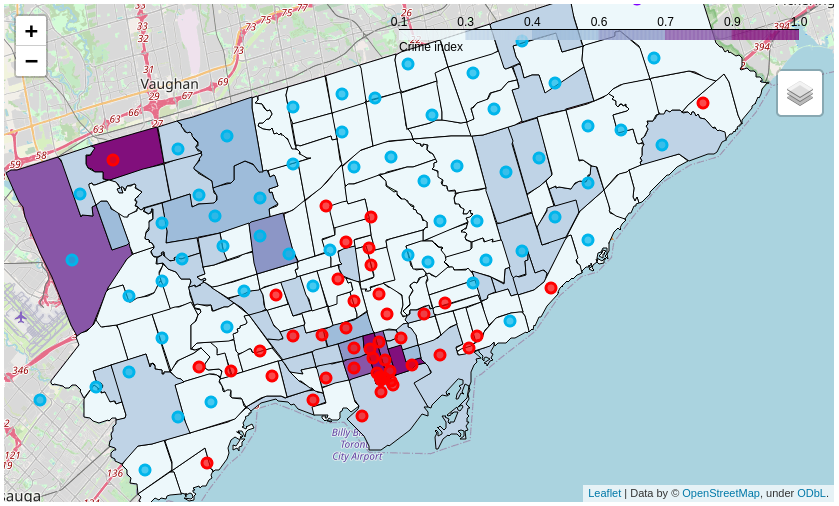
\includegraphics[width=\textwidth]{pics/clustercrime.png}
 \caption{Spatial distribution of crime and of neighbourhood clusters.}\label{fig:clustercrime}
\end{figure}

\subsection{Decision tree and SVM}

\begin{figure}[ht]
     \centering
     \begin{subfigure}[b]{0.47\textwidth}
         \centering
         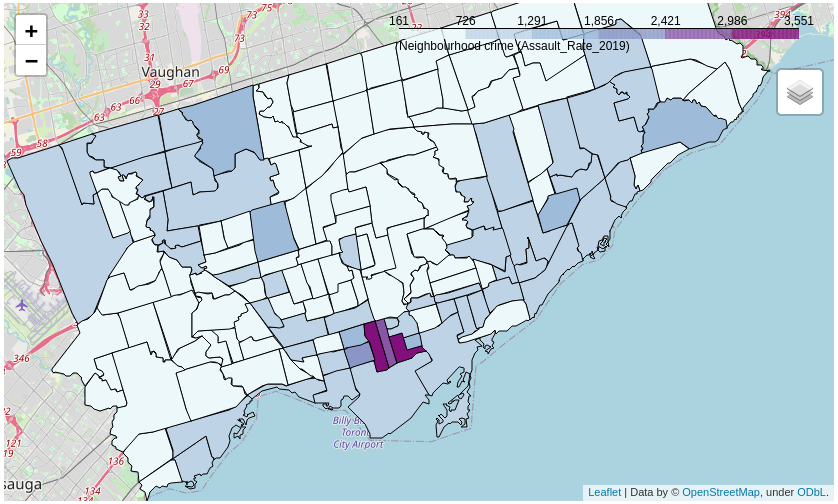
\includegraphics[width=\textwidth]{pics/assault2}
         \caption{Assault}
     \end{subfigure}
     \hfill
     \begin{subfigure}[b]{0.47\textwidth}
         \centering
         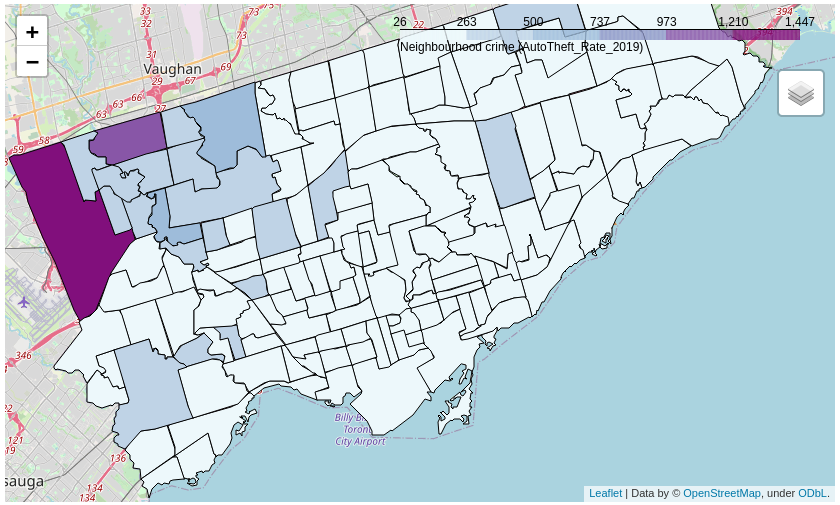
\includegraphics[width=\textwidth]{pics/auto}
         \caption{Auto theft}
     \end{subfigure}
     \begin{subfigure}[b]{0.47\textwidth}
         \centering
         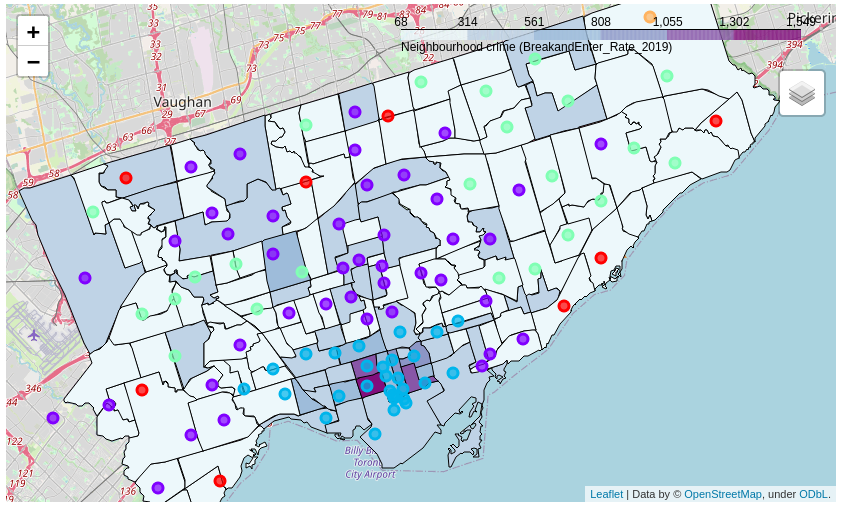
\includegraphics[width=\textwidth]{pics/breakenter}
         \caption{Breaking and entering}
     \end{subfigure}
     \hfill
     \begin{subfigure}[b]{0.47\textwidth}
         \centering
         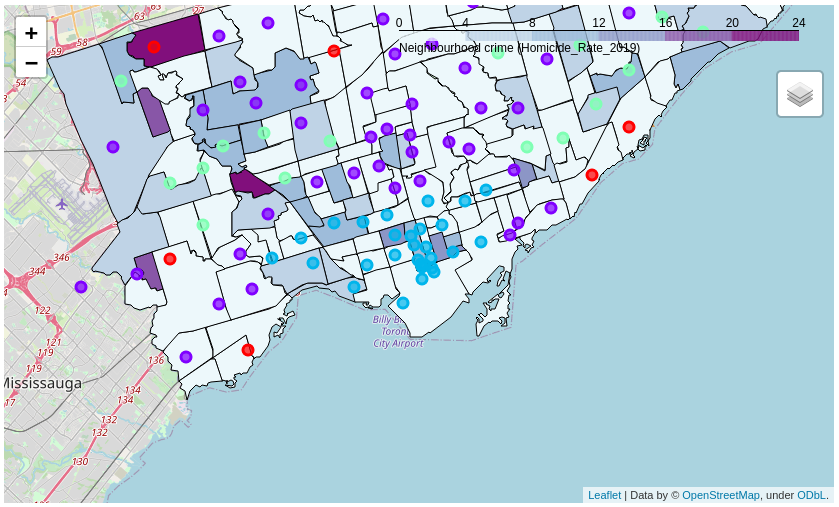
\includegraphics[width=\textwidth]{pics/homicide}
         \caption{Homicide}
     \end{subfigure}
     \begin{subfigure}[b]{0.47\textwidth}
         \centering
         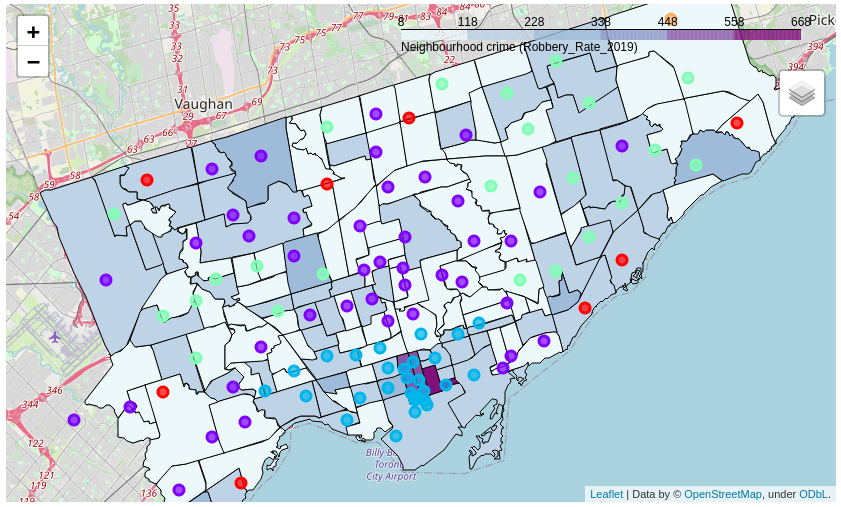
\includegraphics[width=\textwidth]{pics/robbery}
         \caption{Robbery}
     \end{subfigure}
     \hfill
     \begin{subfigure}[b]{0.47\textwidth}
         \centering
         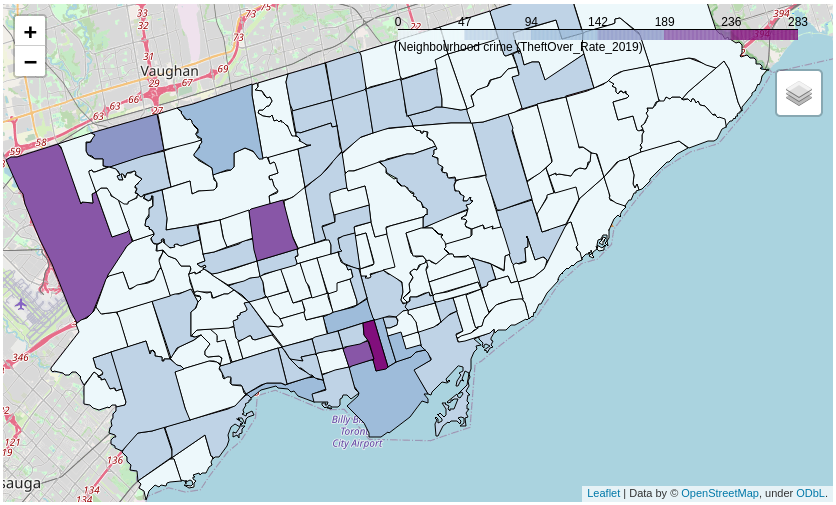
\includegraphics[width=\textwidth]{pics/theftover}
         \caption{Theft other}
     \end{subfigure}
        \caption{The six crime categories, plotted with the five neighbourhood clusters.}
        \label{fig:nbhcrime}
\end{figure}

\section{Discussion}

\section{Conclusion}
 
\end{document}
